\documentclass[10pt]{article}
\usepackage{amsmath}
\usepackage{amsthm}
\usepackage{amsfonts}
\usepackage{dsfont}
\usepackage{amssymb}
\usepackage{latexsym}
\usepackage{tensor}
%\usepackage{epsfig}
\usepackage{graphicx}
\usepackage{tikz}
\usetikzlibrary{cd}
%\usepackage[dvips]{graphicx}
\graphicspath{ {images/} }
\usepackage{pict2e}

\usepackage[matrix,tips,graph,curve]{xy}

\newcommand{\mnote}[1]{${}^*$\marginpar{\footnotesize ${}^*$#1}}
\linespread{1.065}

\makeatletter

\setlength\@tempdima  {5.5in}
\addtolength\@tempdima {-\textwidth}
\addtolength\hoffset{-0.5\@tempdima}
\setlength{\textwidth}{5.5in}
\setlength{\textheight}{8.75in}
\addtolength\voffset{-0.625in}

\makeatother

\makeatletter 
\@addtoreset{equation}{section}
\makeatother


\renewcommand{\theequation}{\thesection.\arabic{equation}}

\theoremstyle{plain}
\newtheorem{theorem}[equation]{Theorem}
\newtheorem{corollary}[equation]{Corollary}
\newtheorem{lemma}[equation]{Lemma}
\newtheorem{proposition}[equation]{Proposition}
\newtheorem{conjecture}[equation]{Conjecture}
\newtheorem{fact}[equation]{Fact}
\newtheorem{facts}[equation]{Facts}
\newtheorem*{theoremA}{Theorem A}
\newtheorem*{theoremB}{Theorem B}
\newtheorem*{theoremC}{Theorem C}
\newtheorem*{theoremD}{Theorem D}
\newtheorem*{theoremE}{Theorem E}
\newtheorem*{theoremF}{Theorem F}
\newtheorem*{theoremG}{Theorem G}
\newtheorem*{theoremH}{Theorem H}

\theoremstyle{definition}
\newtheorem{definition}[equation]{Definition}
\newtheorem{definitions}[equation]{Definitions}
%\theoremstyle{remark}

\newtheorem{remark}[equation]{Remark}
\newtheorem{remarks}[equation]{Remarks}
\newtheorem{exercise}[equation]{Exercise}
\newtheorem{example}[equation]{Example}
\newtheorem{examples}[equation]{Examples}
\newtheorem{notation}[equation]{Notation}
\newtheorem{question}[equation]{Question}
\newtheorem{assumption}[equation]{Assumption}
\newtheorem*{claim}{Claim}
\newtheorem{answer}[equation]{Answer}
%%%%%% letters %%%%

\newcommand{\fA}{\mathfrak{A}}
\newcommand{\fB}{\mathfrak{B}}
\newcommand{\fC}{\mathfrak{C}}
\newcommand{\fD}{\mathfrak{D}}
\newcommand{\fE}{\mathfrak{E}}
\newcommand{\fF}{\mathfrak{F}}
\newcommand{\fG}{\mathfrak{G}}
\newcommand{\fH}{\mathfrak{H}}
\newcommand{\fI}{\mathfrak{I}}
\newcommand{\fJ}{\mathfrak{J}}
\newcommand{\fK}{\mathfrak{K}}
\newcommand{\fL}{\mathfrak{L}}
\newcommand{\fM}{\mathfrak{M}}
\newcommand{\fN}{\mathfrak{N}}
\newcommand{\fO}{\mathfrak{O}}
\newcommand{\fP}{\mathfrak{P}}
\newcommand{\fQ}{\mathfrak{Q}}
\newcommand{\fR}{\mathfrak{R}}
\newcommand{\fS}{\mathfrak{S}}
\newcommand{\fT}{\mathfrak{T}}
\newcommand{\fU}{\mathfrak{U}}
\newcommand{\fV}{\mathfrak{V}}
\newcommand{\fW}{\mathfrak{W}}
\newcommand{\fX}{\mathfrak{X}}
\newcommand{\fY}{\mathfrak{Y}}
\newcommand{\fZ}{\mathfrak{Z}}

\newcommand{\fa}{\mathfrak{a}}
\newcommand{\fb}{\mathfrak{b}}
\newcommand{\fc}{\mathfrak{c}}
\newcommand{\fd}{\mathfrak{d}}
\newcommand{\fe}{\mathfrak{e}}
\newcommand{\ff}{\mathfrak{f}}
\newcommand{\fg}{\mathfrak{g}}
\newcommand{\fh}{\mathfrak{h}}
%\newcommand{\fi}{\mathfrak{i}}

\newcommand{\fj}{\mathfrak{j}}
\newcommand{\fk}{\mathfrak{k}}
\newcommand{\fl}{\mathfrak{l}}
\newcommand{\fm}{\mathfrak{m}}
\newcommand{\fn}{\mathfrak{n}}
\newcommand{\fo}{\mathfrak{o}}
\newcommand{\fp}{\mathfrak{p}}
\newcommand{\fq}{\mathfrak{q}}
\newcommand{\fr}{\mathfrak{r}}
\newcommand{\fs}{\mathfrak{s}}
\newcommand{\ft}{\mathfrak{t}}
\newcommand{\fu}{\mathfrak{u}}
\newcommand{\fv}{\mathfrak{v}}
\newcommand{\fw}{\mathfrak{w}}
\newcommand{\fx}{\mathfrak{x}}
\newcommand{\fy}{\mathfrak{y}}
\newcommand{\fz}{\mathfrak{z}}

\newcommand{\bi}{\textbf{i}}
\newcommand{\bj}{\textbf{j}}
\newcommand{\bk}{\textbf{k}}

\newcommand{\sA}{\mathcal{A}\,}
\newcommand{\sB}{\mathcal{B}\,}
\newcommand{\sC}{\mathcal{C}}
\newcommand{\sD}{\mathcal{D}\,}
\newcommand{\sE}{\mathcal{E}\,}
\newcommand{\sF}{\mathcal{F}\,}
\newcommand{\sG}{\mathcal{G}\,}
\newcommand{\sH}{\mathcal{H}}
\newcommand{\sI}{\mathcal{I}\,}
\newcommand{\sJ}{\mathcal{J}\,}
\newcommand{\sK}{\mathcal{K}\,}
\newcommand{\sL}{\mathcal{L}\,}
\newcommand{\sM}{\mathcal{M}\,}
\newcommand{\sN}{\mathcal{N}}
\newcommand{\sO}{\mathcal{O}}
\newcommand{\sP}{\mathcal{P}\,}
\newcommand{\sQ}{\mathcal{Q}\,}
\newcommand{\sR}{\mathcal{R}}
\newcommand{\sS}{\mathcal{S}}
\newcommand{\sT}{\mathcal{T}\,}
\newcommand{\sU}{\mathcal{U}\,}
\newcommand{\sV}{\mathcal{V}\,}
\newcommand{\sW}{\mathcal{W}\,}
\newcommand{\sX}{\mathcal{X}\,}
\newcommand{\sY}{\mathcal{Y}\,}
\newcommand{\sZ}{\mathcal{Z}\,}

\newcommand{\IA}{\mathbb{A}}
\newcommand{\IB}{\mathbb{B}}
\newcommand{\IC}{\mathbb{C}}
\newcommand{\ID}{\mathbb{D}}
\newcommand{\IE}{\mathbb{E}}
\newcommand{\IF}{\mathbb{F}}
\newcommand{\IG}{\mathbb{G}}
\newcommand{\IH}{\mathbb{H}}
\newcommand{\II}{\mathbb{I}}
\newcommand{\IK}{\mathbb{K}}
\newcommand{\IL}{\mathbb{L}}
\newcommand{\IM}{\mathbb{M}}
\newcommand{\IN}{\mathbb{N}}
\newcommand{\IO}{\mathbb{O}}
\newcommand{\IP}{\mathbb{P}}
\newcommand{\IQ}{\mathbb{Q}}
\newcommand{\IR}{\mathbb{R}}
\newcommand{\IS}{\mathbb{S}}
\newcommand{\IT}{\mathbb{T}}
\newcommand{\IU}{\mathbb{U}}
\newcommand{\IV}{\mathbb{V}}
\newcommand{\IW}{\mathbb{W}}
\newcommand{\IX}{\mathbb{X}}
\newcommand{\IY}{\mathbb{Y}}
\newcommand{\IZ}{\mathbb{Z}}

 \newcommand{\tA}{\mathrm {A}}
 \newcommand{\tB}{\mathrm {B}}
 \newcommand{\tC}{\mathrm {C}}
 \newcommand{\tD}{\mathrm {D}}
 \newcommand{\tE}{\mathrm {E}}
 \newcommand{\tF}{\mathrm {F}}
 \newcommand{\tG}{\mathrm {G}}
 \newcommand{\tH}{\mathrm {H}}
 \newcommand{\tI}{\mathrm {I}}
 \newcommand{\tJ}{\mathrm {J}}
 \newcommand{\tK}{\mathrm {K}}
 \newcommand{\tL}{\mathrm {L}}
 \newcommand{\tM}{\mathrm {M}}
 \newcommand{\tN}{\mathrm {N}}
 \newcommand{\tO}{\mathrm {O}}
 \newcommand{\tP}{\mathrm {P}}
 \newcommand{\tQ}{\mathrm {Q}}
 \newcommand{\tR}{\mathrm {R}}
 \newcommand{\tS}{\mathrm {S}}
 \newcommand{\tT}{\mathrm {T}}
 \newcommand{\tU}{\mathrm {U}}
 \newcommand{\tV}{\mathrm {V}}
 \newcommand{\tW}{\mathrm {W}}
 \newcommand{\tX}{\mathrm {X}}
 \newcommand{\tY}{\mathrm {Y}}
 \newcommand{\tZ}{\mathrm {Z}}
%%%%%%% macros %%%%%

%% my definitions %%%

\newcommand{\End}{\mathrm{End}}
\newcommand{\tr}{\mathrm{tr}}
%\newcommand{\ind}{\mathrm{ind}}

\renewcommand{\index}{\mathrm{index \,}}
\newcommand{\Hom}{\mathrm{Hom}}
\newcommand{\Aut}{\mathrm{Aut}}
\newcommand{\Trace}{\mathrm{Trace}\,}
\newcommand{\Res}{\mathrm{Res}\,}
\newcommand{\rank}{\mathrm{rank}}
%\renewcommand{\dim}{\mathrm{dim}}

\renewcommand{\deg}{\mathrm{deg}}
\newcommand{\spin}{\rm Spin}
\newcommand{\Spin}{\rm Spin}
\newcommand{\erfc}{\rm erfc\,}
\newcommand{\sgn}{{\rm sgn\,}}
\newcommand{\Spec}{\rm Spec\,}
\newcommand{\diag}{\rm diag\,}
\newcommand{\Fix}{\mathrm{Fix}}
\newcommand{\Ker}{\mathrm{Ker \,}}
\newcommand{\Coker}{\mathrm{Coker \,}}
\newcommand{\Sym}{\mathrm{Sym \,}}
\newcommand{\Hess}{\mathrm{Hess \,}}
\newcommand{\grad}{\mathrm{grad \,}}
\newcommand{\Center}{\mathrm{Center}}
\newcommand{\Lie}{\mathrm{Lie}}


\newcommand{\ch}{\rm ch} % Chern Character

\newcommand{\rk}{\rm rk} 
%\renewcommand{\c}{\rm c}  % Chern class

\newcommand{\sign}{\rm sign}
\renewcommand\dim{{\rm dim\,}}
\renewcommand\det{{\rm det\,}}
\newcommand{\dimKrull}{{\rm Krulldim\,}}
\newcommand\Rep{\mathrm{Rep}}
\newcommand\Hilb{\mathrm{Hilb}}
\newcommand\vol{\mathrm{vol}}

\newcommand\QED{\hfill $\Box$} %{\bf QED}} 

\newcommand\Pf{\nonintend{\em Proof. }}


\newcommand\reals{{\mathbb R}} 
\newcommand\complexes{{\mathbb C}}
\renewcommand\Re{\mathrm Re}
\renewcommand\Im{\mathrm Im}
\newcommand\integers{{\mathbb Z}}
\newcommand\quaternions{{\mathbb H}}


\newcommand\iso{{\cong}} 
%\newcommand\tensor{{\otimes}}
\newcommand\Tensor{{\bigotimes}} 
\newcommand\union{\bigcup} 
\newcommand\onehalf{\frac{1}{2}}
%\newcommand\Sym[1]{{Sym^{#1}(\complexes^2)}}

\newcommand\lie[1]{{\mathfrak #1}} 
\renewcommand\fk{\mathfrak{K}}
\newcommand\smooth{\mathcal{C}^{\infty}}
\newcommand\trivial{{\mathbb I}}
\newcommand\widebar{\overline}

%%%%%Delimiters%%%%

\newcommand{\<}{\langle}
\renewcommand{\>}{\rangle}

%\renewcommand{\(}{\left(}
%\renewcommand{\)}{\right)}


%%%% Different kind of derivatives %%%%%

\newcommand{\delbar}{\bar{\partial}}
\newcommand{\pdu}{\frac{\partial}{\partial u}}
%\newcommand{\pd}[1][2]{\frac{\partial #1}{\partial #2}}

%%%%% Arrows %%%%%
%\renewcommand{\ra}{\rightarrow}                   % right arrow
%\newcommand{\lra}{\longrightarrow}              % long right arrow
%\renewcommand{\la}{\leftarrow}                    % left arrow
%\newcommand{\lla}{\longleftarrow}               % long left arrow
%\newcommand{\ua}{\uparrow}                     % long up arrow
%\newcommand{\na}{\nearrow}                      %  NE arrow
%\newcommand{\llra}[1]{\stackrel{#1}{\lra}}      % labeled long right arrow
%\newcommand{\llla}[1]{\stackrel{#1}{\lla}}      % labeled long left arrow
%\newcommand{\lua}[1]{\stackrel{#1}{\ua}}      % labeled  up arrow
%\newcommand{\lna}[1]{\stackrel{#1}{\na}}      % labeled long NE arrow

\newcommand{\into}{\hookrightarrow}
\newcommand{\tto}{\longmapsto}
\def\llra{\longleftrightarrow}

\def\d/{/\mspace{-6.0mu}/}
\newcommand{\git}[3]{#1\d/_{\mspace{-4.0mu}#2}#3}
\newcommand\zetahilb{\zeta_{{\text{Hilb}}}}
\def\Fy{\sF \mspace{-3.0mu} \cdot \mspace{-3.0mu} y}
\def\tv{\tilde{v}}
\def\tw{\tilde{w}}
\def\wt{\widetilde}
\def\wtilde{\widetilde}
\def\what{\widehat}

%%%%%%%%%%%%%%%%%%% Mark's definitions %%%%%%%%%%%%%%%%%%%%

\newcommand{\frakg}{\mbox{\frakturfont g}}
\newcommand{\frakk}{\mbox{\frakturfont k}}
\newcommand{\frakp}{\mbox{\frakturfont p}}
\newcommand{\q}{\mbox{\frakturfont q}}
\newcommand{\frakn}{\mbox{\frakturfont n}}
\newcommand{\frakv}{\mbox{\frakturfont v}}
\newcommand{\fraku}{\mbox{\frakturfont u}}
\newcommand{\frakh}{\mbox{\frakturfont h}}
\newcommand{\frakm}{\mbox{\frakturfont m}}
\newcommand{\frakt}{\mbox{\frakturfont t}}
\newcommand{\G}{\Gamma}
\newcommand{\g}{\gamma}
\newcommand{\fraka}{\mbox{\frakturfont a}}
\newcommand{\db}{\bar{\partial}}
\newcommand{\dbs}{\bar{\partial}^*}
\newcommand{\p}{\partial}

%%%%%%%%%%%%% new definitions for the positive mass paper %%%%%%%%%

\newcommand{\sperp}{{\scriptscriptstyle \perp}}

%%%%%%%%%%%%%%%%%%%%%%%



%%%%%%%%%%%%%%%%%%%%%%%%%%%%%%%%%%%%%%%%%%%%%

%%%%%%%%%%%%%%%%%%%%%%
% macreau for tableaux
%%%%%%%%%%%%%%%%%%%%%%
\newlength\cellsize \setlength\cellsize{8\unitlength}

\savebox2{% BOX
\begin{picture}(8,8)
\put(0,0){\line(1,0){8}}
\put(0,0){\line(0,1){8}}
\put(8,0){\line(0,1){8}}
\put(0,8){\line(1,0){8}}
\end{picture}}

\newcommand\boxify[1]{\def\thearg{#1}\def\nothing{}%
\ifx\thearg\nothing\vrule width0pt height\cellsize depth0pt%
  \else\hbox to 0pt{\usebox2\hss}\fi%
  \vbox to \cellsize{\vss\hbox to \cellsize{\hss$_{#1}$\hss}\vss}}

\savebox3{% CIRCLE
\begin{picture}(8,8)
\put(4,4){\circle{8}}
\end{picture}}

\savebox4{% CROSS
\begin{picture}(8,8)
\put(2,0){\line(1,2){4}}
\put(6,0){\line(-1,2){4}}
\end{picture}}



\savebox7{% DOT
\begin{picture}(8,8)
\put(4,4){\circle*{3}}
\end{picture}}



\newcommand{\circify}[1]{\def\thearg{#1}\def\nothing{}%
\ifx\thearg\nothing\vrule width0pt height\cellsize depth0pt%
  \else\hbox to 0pt{\usebox3\hss}\fi%
  \vbox to \cellsize{\vss\hbox to \cellsize{\hss$_{#1}$\hss}\vss}}

\newcommand\nullify[1]{\def\thearg{#1}\def\nothing{}%
\ifx\thearg\nothing\vrule width0pt height\cellsize depth0pt%
  \else\hbox to 0pt{\hss}\fi%
  \vbox to \cellsize{\vss\hbox to \cellsize{\hss$_{#1}$\hss}\vss}}


\newcommand\tableau[1]{\vtop{\let\\=\cr
\setlength\baselineskip{-8000pt}
\setlength\lineskiplimit{8000pt}
\setlength\lineskip{0pt}
\halign{&\boxify{##}\cr#1\crcr}}}

\newcommand\cirtab[1]{\vline\vtop{\let\\=\cr
\setlength\baselineskip{-8000pt}
\setlength\lineskiplimit{8000pt}
\setlength\lineskip{0pt}
\halign{&\circify{##}\cr#1\crcr}}}

\newcommand\nulltab[1]{\vtop{\let\\=\cr
\setlength\baselineskip{-8000pt}
\setlength\lineskiplimit{8000pt}
\setlength\lineskip{0pt}
\halign{&\nullify{##}\cr#1\crcr}}}

\newcommand\boxtab[1]{\vline\vtop{\let\\=\cr
\setlength\baselineskip{-8000pt}
\setlength\lineskiplimit{8000pt}
\setlength\lineskip{0pt}
\halign{&\nullify{##}\cr#1\crcr}}}


\newcommand{\cball}{%
  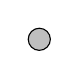
\begin{tikzpicture}
    \filldraw[fill=black!25,draw=black] circle (4pt);
  \end{tikzpicture}
}




%
\begin{document}
%

\title{Characterizing Permutation Bubble Diagrams}
\author{Ben Gillen and Jonathan Michala}


\date{\today}

\maketitle
\section{Introduction}
Consider a permutation $w = w_1w_2...w_n$ in the symmetric group $\fS_n$.
An \textbf{\textit{inversion}} of $w$ is a pair of indices $i < j$ such that $w_i > w_j$.
For example, if $w = 152869347 \in \fS_9$, then $w_4 = 8$ and $w_7 = 3$ would be an inversion.
One way to visualize inversions is with the \textbf{\textit{Rothe Diagram}} of $w$, defined to be the following subset of cells in the first quadrant \cite{inversion}:
\begin{equation}
\ID(w) = \{(i,w_j) \colon i < j, w_i > w_j\} \subset \IZ^+ \times \IZ^+.
\end{equation}

Graphically, we represent cells in $\ID(w)$ by bubbles and use the convention that the $i$ coordinates are written on the vertical axis and the $w_j$ coordinates are written on the horizontal axis. 

Equivalently, the Rothe Diagram can be visualized as the bubbles not touched by lines originating at each $(i,w_i)$, where each line extends either up or to the right.

\begin{example}
Consider the first Rothe diagram $\ID(152869347)$, shown in Figure \ref{fig:rothe}. There is a bubble at $(4,3)$ for example, because $i = 4 < 7 = j$ and $w_i = 8 > 3 = w_j$. The second Rothe diagram in \ref{fig:rothe} gives the alternate visualization. Vertical and horizontal lines extend out from each $(i,w_i)$, e.g. for $i=3, w_3=2$, a pair of lines extends out from $(3,2)$.

\begin{figure}
\begin{center}
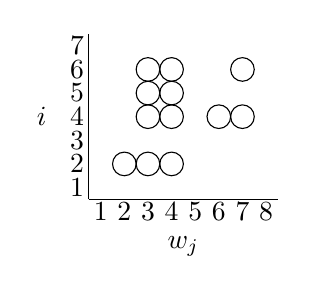
\begin{tikzpicture}[scale=0.3]
\def\rows{8} %number of rows
\def\cols{7} %number of columns
  \draw[-](0,0) -- (\rows,0); %axes
  \draw[-](0,0) -- (0,\cols); 
  \foreach \y in {1,2,...,\cols} %labels
    \draw (-0.5,\y-0.5) node{\y}; 
  \draw (-2,\cols / 2) node{$i$};
  \foreach \x in {1,2,...,\rows}
    \draw (\x-0.5,- 0.5) node{\x};
  \draw (\rows / 2,-2) node{$w_j$}; 
  \foreach \x/\y in {2/2,3/2,4/2,3/4,4/4,6/4,7/4,3/5,4/5,3/6,4/6,7/6} %positions
    \draw (\x-0.5,\y-0.5) circle(0.5);
\end{tikzpicture}

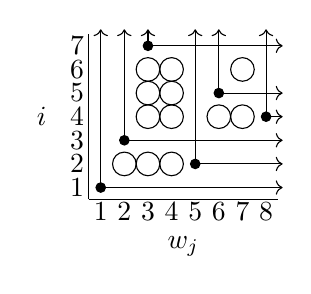
\begin{tikzpicture}[scale=0.3]
\def\rows{8} %number of rows
\def\cols{7} %number of columns
  \draw[-](0,0) -- (\rows,0); %axes
  \draw[-](0,0) -- (0,\cols); 
  \foreach \y in {1,2,...,\cols} %labels
    \draw (-0.5,\y-0.5) node{\y}; 
  \draw (-2,\cols / 2) node{$i$};
  \foreach \x in {1,2,...,\rows}
    \draw (\x-0.5,- 0.5) node{\x};
  \draw (\rows / 2,-2) node{$w_j$}; 
  \foreach \x/\y in {1/1,2/3,3/7,5/2,6/5,8/4} %dot positions
    \draw[fill=black] (\x-0.5,\y-0.5) circle(0.2);
  \foreach \x/\y in {1/1,2/3,3/7,5/2,6/5,8/4} %vertical lines
    \draw[->](\x-0.5,\y-0.5) -- (\x-0.5,7.2);
  \foreach \x/\y in {1/1,2/3,3/7,5/2,6/5,8/4} %horizontal lines
    \draw[->](\x-0.5,\y-0.5) -- (8.2,\y-0.5); 
  \foreach \x/\y in {2/2,3/2,4/2,3/4,4/4,6/4,7/4,3/5,4/5,3/6,4/6,7/6} %positions
    \draw (\x-0.5,\y-0.5) circle(0.5);
\end{tikzpicture}
\caption{\label{fig:rothe} The Rothe Diagram $\ID(152869347)$, visualized through two methods.}
\end{center}
\end{figure}

\end{example}

Rothe Diagrams satisfy many properties, and this paper discusses which properties are sufficient for an arbitrary diagram $D \subset \IZ^+ \times \IZ^+$ to be the Rothe Diagram of some permutation.
(Note that Rothe Diagrams have a finite number of bubbles, so unless otherwise stated, we assume any $D \subset \IZ^+ \times \IZ^+$ also has a finite number of bubbles).
In the second section we show several properties satisfied by Rothe Diagrams, and in the third section, we prove several characterizations of Rothe Diagrams with these properties.

\section{Properties of Permutation Diagrams}

\textbf{todo: thinking we use the three examples (main diagram, and two-bubble diagonal diagrams) for each property and have the three diagrams in one figure for each.}

\begin{definition}
Assume a column of bubbles in the zero-th column.
\[ (0,w_j) = 1 \; \forall j \in \IZ_+ \]
These bubbles are labelled \textbf{\textit{addendum bubbles}} and are always appended to a diagram when considering the rules below. However, these bubbles are not counted towards the total number of bubbles in each row.
\end{definition}

\begin{figure}[ht]
  \begin{displaymath}
    \arraycolsep=0.9\cellsize
    \begin{array}{cc}
      \nulltab{
        \cball \\
        \cball \\
        \cball \\
        \cball \\
        \cball \\
        \cball \\
      }
      \cirtab{ 
        & & \ & \ & & & \ \\
        & & \ & \ \\
        & & \ & \ & & \ & \ \\
        & & \\
        & \ & \ & \ \\ & \\\hline } &
      
    \end{array}
  \end{displaymath}
  \caption{\label{fig:addendum}The main diagram with the addendum bubbles shaded.}
\end{figure}


\begin{definition}
The \textbf{\textit{final bubble}} is defined as the last bubble in a row, where all cells afterwards are empty. Final bubbles will be counted with the following function. It returns a $1$ if the final bubble is at the $(i, w_j)$ location and a $0$ otherwise.
\[ R_{(i,w_j)} =  \begin{cases} 
1 & (i,w_j) = 1 \mid (n,w_j) = 0 \quad \forall n > i \\
0 & \text{otherwise}
\end{cases} \]
Since the addendum bubble exists, each row must contain a final bubble.
\end{definition}

\begin{figure}[ht]
  \begin{displaymath}
    \arraycolsep=0.9\cellsize
    \begin{array}{cc}
      \nulltab{
        \usebox3 \\
        \usebox3 \\
        \usebox3 \\
        \cball \\
        \usebox3 \\
        \cball \\
      }
      \cirtab{ 
        & & \ & \ & & & \cball \\
        & & \ & \cball \\
        & & \ & \ & & \ & \cball \\
        & & \\
        & \ & \ & \cball \\ & \\\hline } &
      
    \end{array}
  \end{displaymath}
  \caption{\label{fig:finals}The main diagram with the final bubbles shaded.}
\end{figure}

\begin{definition}
\textbf{todo: could define this in terms of row dots, which are defined for the dot condition}
The \textbf{\textit{vertical ascension}} rule states that the cells in the column in or above the first cell after the final bubble in a row such that no other similar column yet exists in that row must be empty. Specifically, consider a cell $(\ell,w_j)$ which contains a final bubble. Let column $\ell$ contain $m_0$ final bubbles below row $w_j$. If the $m_0$ columns to the right of column $\ell$ contain $0$ final bubbles (below row $w_j$), then the vertical ascension rule picks out the $(1+\ell+m_0,w_j)$ cell. There are no bubbles in that cell or in the column above it. If there are $m_1 > 0$ final bubbles in this range, repeat the process. Since permutations considered in this paper are finite, for some $z$ there will be $0$ final bubbles in the $m_{z}$ columns to the right of the $\ell + \sum_{s=0}^{z-1} m_s$ column (below row $w_j$). Then, the $(1+ \ell + \sum_{s=0}^{z} m_s, w_j)$ cell must be empty and so must all cells in the same column above the $w_j$ row.
\[
  \sum_{q=\ell+\mu-m_z}^{\ell+\mu} \, \sum_{r=1}^{j-1} R_{(q,w_r)} = 0 \implies (1+\ell+\mu,w_p) = 0 \quad \quad p \geq j, \; \mu = \sum_{s=0}^{z} m_s
\]

\end{definition}


\begin{figure}[ht]
  \begin{displaymath}
    \arraycolsep=0.9\cellsize
    \begin{array}{ccc}
      \nulltab{
                \\
        \usebox3 \\
        \usebox3 \\
        \usebox3 \\
        \cball \\
        \usebox3 \\
        \cball \\
      }
      \boxtab{ 
        
        & & & & & & & & \put(0,0){\vector(0,1){10}} \\
        & & \usebox3 & \usebox3 & & \put(0,0){\vector(0,1){10}} & \cball & & \usebox4 \\
        & & \usebox3 & \cball & & \usebox4 & & \put(0,0){\vector(0,1){10}} \\
        & \put(0,0){\vector(0,1){10}} & \usebox3 & \usebox3 & & \usebox3 & \cball & \usebox4 \\
        & \usebox4 & & & \put(0,0){\vector(0,1){10}} \\
        \put(0,0){\vector(0,1){10}} & \usebox3 & \usebox3 & \cball & \usebox4 \\ 
        \usebox4 & \\\hline }

      
    \end{array}
  \end{displaymath}
  \caption{\label{fig:main_va}The main diagram with the vertical ascension rule applied.}
\end{figure}

\begin{proposition}
Permutation diagrams satisfy the vertical ascension rule.
\end{proposition}

\begin{proof}
Take column $\ell$ with a final bubble in row $w_j$ and $m_0$ final bubbles below row $w_j$. Each of these final bubbles below row $w_j$ corresponds to a death ray. There must be a death ray in each of the succeeding $\sum_{s=0}^{z} m_s$ columns after column $\ell$ where
\[
\sum_{q=\ell+\mu-m_z}^{\ell+\mu} \, \sum_{r=1}^{j-1} R_{(q,w_r)} = 0 \quad \quad \mu = \sum_{s=0}^{z} m_s
\]
because multiple death rays are not allowed to be placed in the same column. For each $m_i$ final bubbles added, the death ray in row $w_j$ cannot be placed in the next $m_i$ columns, as each of those columns must already be filled by a death ray. Each death ray extends infinitely upwards, preventing bubbles from being placed in the column above them. The final bubble $(\ell,w_j)$ corresponds to a new death ray being placed in the $(1+\ell+\sum_{s=1}^{z} m_s, w_j)$ cell. The vertical ascension rule is identical in disallowing bubbles from the exact same cells. Therefore, the vertical ascension rule is satisfied in permutation diagrams.
\end{proof}

\begin{figure}[ht]
  \begin{displaymath}
    \arraycolsep=0.9\cellsize
    \begin{array}{cc}
      \nulltab{
      \\
        \usebox3 \\
        \cball \\
        \usebox3 \\
        \usebox3 \\
      }
      \boxtab{ 
        & & & & & \put(0,0){\vector(0,1){10}} \\
        \put(0,0){\vector(0,1){10}} & & &  & \cball & \usebox4 \\
        \usebox4 & \put(0,0){\vector(0,1){10}} \\
        \cball & \usebox4 & \put(0,0){\vector(0,1){10}} \\
        \usebox3 & \cball & \usebox4 \\\hline } &
      
    \end{array}
  \end{displaymath}
  \caption{\label{fig:bad_va}A bubble diagram which satisfies the vertical ascension rule, but is not a permutation diagram.}
\end{figure}

\begin{definition}
For $D \subset \IZ^+ \times \IZ^+$, define \textbf{\textit{row dots}} $R(D) = \{(1,w_1),(2,w_2),...\}$ in $\IZ^+ \times \IZ^+$ such that $(i,w_i)$ is the first position to the right of all the bubbles in the $i$th row that satisfies $w_i \neq w_j$ for all $j < i$.
Similarly, define \textbf{\textit{column dots}} $C(D) = \{(i_1,1),(i_2,2),...\}$ in $\IZ^+\times \IZ^+$ such that $(i_w,w)$ is the first position above all the bubbles in the $w$th column that satisfies $i_w \neq i_v$ for all $v < w$.
We say that a diagram satisfies the \textbf{\textit{dot rule}} and is a \textbf{\textit{dotted diagram}} if $R(D) = C(D)$.
\end{definition}

\begin{figure}
\begin{center}
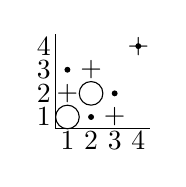
\begin{tikzpicture}[scale=0.3]
\def\rows{4}
\def\cols{4}
  \draw[-](0,0) -- (\rows,0);
  \draw[-](0,0) -- (0,\cols);
  \foreach \y in {1,2,...,\cols}
    \draw (-0.5,\y-0.5) node{\y};
  \foreach \x in {1,2,...,\rows}
    \draw (\x-0.5,- 0.5) node{\x};
  \foreach \x/\y in {1/1,2/2}
    \draw (\x-0.5,\y-0.5) circle(0.5);
  \foreach \x/\y in {2/1,3/2,1/3,4/4}
    \filldraw (\x-0.5,\y-0.5) circle(0.1);
  \foreach \x/\y in {1/2,2/3,3/1,4/4}
    \draw (\x-0.5,\y-0.5) node{+};
\end{tikzpicture}
\caption{\label{fig:dot_ex} A diagram $D$ with $R(D) \neq C(D)$, shown by dots and plus signs respectively}
\end{center}
\end{figure}


\begin{figure}[ht]
  \begin{displaymath}
    \arraycolsep=0.9\cellsize
    \begin{array}{cc}
      \boxtab{ 
        & & \usebox3 & \usebox3 & & & \usebox3 & & \usebox7 \\
        & & \usebox3 & \usebox3 & & \usebox7 \\
        & & \usebox3 & \usebox3 & & \usebox3 & \usebox3 & \usebox7 \\
        & \usebox7 & \\
        & \usebox3 & \usebox3 & \usebox3 & \usebox7 \\
        \usebox7 & \\\hline } &
      
    \end{array}
  \end{displaymath}
    \caption{\label{fig:main_dot}The main diagram with the dot condition applied.}
\end{figure}

\begin{proposition}
Permutation diagrams satisfy the dot condition
\end{proposition}

\begin{proof}
In both procedures, we place dots exactly in the locations $(i,w_i)$ for all $i \in \IZ_+$.
In the first procedure, in the first row, we place bubbles in all the cells $(1,w_j)$ such that $1 < j$ and $w_1 > w_j$.
We know these two conditions are true for the first cells $(1,1),(1,2),...,(1,w_1 - 2),(1,w_1-1)$ and becomes false for $(1,w_1)$, which is therefore where the dot in this row must be placed by the dot procedure.
For the $k$th row, consider any cell $(k,w_j)$.
If $k > j$, then there is a dot at $(j,w_j)$ below the $k$th row and so there cannot be a dot in $(k,w_j)$ by the rules of the procedure.
If $w_k < w_j$, then $(k,w_k)$ is to the left of $(k,w_j)$ and would get a dot before $(k,w_j)$ according to the procedure, so there is no dot in $(k,w_j)$.
This is because we know there is no dot below $(k,w_k)$ by induction on the previous rows.
And if $k < j$ and $w_k > w_j$, then there is a bubble in this $(k,w_j)$.
Hence, if $j \neq k$, then there is no dot in the $(k,w_j)$th cell, and therefore the only cell in which a dot can be placed by the procedure is $(k,w_k)$.

In the second procedure, in the first column, we place bubbles in all the cells $(i,1)$ such that $i < j$ and $w_i > 1$ for $j$ the index giving $w_j = 1$.
We know these two conditions are true for the first cells $(1,1)(2,1),...,(j-2,1),(j-1,1)$ and becomes false for $(j,1)$ which is therefore where the dot in this column must be placed by this dot procedure.
For the $w_k$th column, consider any cell $(i,w_k)$.
If $i < k$ and $w_i > w_k$, then there is a bubble in this cell.
If $i > k$ then $(k,w_k)$ is below $(i,w_k)$ and would get a dot before $(i,w_k)$ by the procedure, so there is no dot in $(i,w_k)$.
This is because we know there is no dot to the left of $(k,w_k)$ by induction on the previous columns.
If $w_i < w_k$, then there is a dot at $(i,w_i)$ to the left of the $w_k$th column and so there cannot be a dot in $(i,w_k)$ by the rules of the procedure.
Hence, if $i \neq k$, then there is no dot in the $(i,w_k)$th cell, and therefore the only cell in which a dot can be placed by the procedure is $(k,w_k)$.

We have then shown that all dots are placed in the same cells by both procedures, so any permutation bubble diagram satisfies the dot condition.
\end{proof}

\begin{figure}[ht]
  \begin{displaymath}
    \arraycolsep=0.9\cellsize
    \begin{array}{cc}
      \boxtab{ 
        & & \usebox7 \\
        & \usebox7 & \\
        \usebox7 & & \\
        \usebox3 & \usebox3 & \usebox3 & \usebox7 & \\
        & & & \usebox3 & \usebox7 \\\hline } &
      
    \end{array}
  \end{displaymath}
  \caption{\label{fig:bad_dot}A bubble diagram which satisfies the dot condition, but is not a permutation diagram.}
\end{figure}

\begin{definition}
Consider a bubble $(i, w_j) = 1$ that is succeeded by $n$ empty cells 
\[(i+k, w_j) = 0 \quad \forall k \leq n, \quad k,n \in \IZ_+ \]
and a bubble after these empty cells $(i+(n+1), w_{j}) = 1$. Take a box bounded by the two aforementioned bubbles and the bottom of the diagram. Remove the rightmost column and topmost row.
\[ \mathcal{B}_{(i+(n+1), w_{j})} = ([i,i+n], [1,w_{j-1}]) \]
%\[ \mathcal{B}_{(i+(n+1), w_{j})} = [(i, w_{j-1}),(i,1)] \times [(i,w_{j-1}), (i+n, w_{j-1})] \]
The \textbf{\textit{empty cell gap}} rule states there are exactly $n$ final bubbles contained within box $\mathcal{B}$.
\end{definition}

\begin{figure}[ht]
  \begin{displaymath}
    \arraycolsep=0.9\cellsize
    \begin{array}{ccc}
      \nulltab{
        \\
        \\
        \\
        \put(4,0){\line(0,1){8}} \\
        \put(4,0){\line(0,1){8}} \\
        \put(4,0){\line(0,1){8}} \\
      }
      \nulltab{
        \usebox3 \\
        \usebox3 \\
        \usebox3 \put(-8,0){\line(1,0){9}} \\
        \cball \\
        \usebox3 \put(-8,0){\line(1,0){9}} \\
        \cball \put(-8,0){\line(1,0){9}} \\
      }
      \boxtab{ 
        
        & & \usebox3 & \usebox3 \put(-8,0){\line(1,0){8}} & \put(-4,-6.5){\line(1,0){8}} & \put(-4,-6.5){\line(1,0){8}} & \cball & & \\
        & & \usebox3 & \put(0.2,0){\line(0,1){8.5}} \cball & & d & \put(-4,0){\line(0,1){8}} & \\
        \put(-4,-6.5){\line(1,0){8}} & \put(-4,-6.5){\line(1,0){8}} & \usebox3 & \put(0,0){\line(0,1){8}} \usebox3 \put(-8,0){\line(1,0){8}} & \put(-4,-6.5){\line(1,0){8}} & \usebox3 & \put(0.2,0){\line(0,1){9}} \cball & \\
        & b & \put(-4,0){\line(0,1){8}} & \put(-4,0){\line(0,1){8}} & c & \put(-4,0){\line(0,1){8}} & \put(-4,0){\line(0,1){8}} \\
        \put(-4,-6.5){\line(1,0){8}} & \usebox3 & \put(0,0){\line(0,1){8}} \usebox3 & \put(0.2,0){\line(0,1){9}} \cball & & \put(-4,0){\line(0,1){8}} & \put(-4,0){\line(0,1){8}} \\ 
        a & \put(-4,0){\line(0,1){8}} & \put(-4,0){\line(0,1){8}} & \put(-4,0){\line(0,1){8}} & & \put(-4,0){\line(0,1){8}} & \put(-4,0){\line(0,1){8}} \\\hline }
      
    \end{array}
  \end{displaymath}
  \caption{\label{fig:ecg_main}The main diagram showing the empty cell gap rule is satisfied. In this example, box $a = \mathcal{B}_{(2, 2)}$ is generated by a gap of length one and contains one final bubble. Box $b = \mathcal{B}_{(4, 3)}$, box $c = \mathcal{B}_{(4, 6)}$, and box $d = \mathcal{B}_{(7, 7)}$ likewise have the same number of final bubbles as the lengths of their gaps. Two of the six empty cell gap boxes are omitted, i.e. $\mathcal{B}_{(5, 3)}$ and $\mathcal{B}_{(6, 3)}$. This choice was to keep the graph uncluttered and readable, but it should be noted that these two gaps also need to be checked.}
\end{figure}

\begin{proposition}
Permutation diagrams satisfy the empty cell gap rule.
\end{proposition}

\begin{proof}
Assume a bubble in the cell $(i_1,w_{j})$ and $(i_2+1, w_{j})$, where the $((i_2+1) - i_1) = n$ cells in between are all empty. The permutation diagram requires exactly $n$ death rays to begin between the $i_1$ and $i_2+1$ columns and below the $w_{j}$ row. Given that the $(i_1,w_{j})$ bubble exists,  a death ray cannot be located in the $i_1$ column below the $w_{j}$ row. Therefore, for every death ray beginning between the $i_1$ and $i_2+1$ columns, a final bubble is contained in the $i_1$ to $i_2-1$ column range. So, the empty cell gap rule is satisfied by permutation diagrams.
\end{proof}

\textbf{TODO: Show example diagram satisfying the ECG rule but is not a permutation diagram. Also, possibly show examples why the final bubble must be in the $i_1$ to $i_2-1$ range?}

\begin{definition}
Consider two procedures for labeling the bubbles in a bubble diagram with numbers.
First, we give the bubbles a \textbf{\textit{horizontal numbering}} where in the $i$th row, we label the bubbles from left to right $i,i+1,i+2,$ and so on.
Second, we give the bubbles a \textbf{\textit{vertical numbering}} where in the $j$th column, we label the bubbles from bottom to top $j,j+1,j+2,$ and so on.
We say a bubble diagram satisfies the \textbf{\textit{numbering condition}} and is a \textbf{\textit{numbered diagram}} if the horizontal numbering and vertical numbering yield the same labels for each bubble.
\end{definition}

\begin{figure}[ht]
  \begin{displaymath}
    \arraycolsep=0.9\cellsize
    \begin{array}{c}
      \cirtab{ 
        & & 6 & 7 & & & 8 \\
        & & 5 & 6 \\
        & & 4 & 5 & & 6 & 7 \\
        & & \\
        & 2 & 3 & 4 \\
        & \\\hline}
      
    \end{array}
    \begin{array}{c}
      \cirtab{
        & 2 \\
        1 & \\\hline}
    \end{array}
    \begin{array}{c}
      \cirtab{
        2 & \\
        & 1 \\\hline}
    \end{array}
    \begin{array}{c}
      \cirtab{
        1 & \\
        & 2 \\\hline}
    \end{array}
  \end{displaymath}
  \caption{\label{fig:main_number} $\ID(152869347)$ satisfies the numbering condition.
  The second diagram also satisfies the numbering condition but is not a Rothe Diagram.
  The third and fourth diagrams show a different horizontal and vertical numbering for the same diagram, so it doesn't satisfy the numbering condition.
  \textbf{todo: numbers labeling the axes here?, line up on bottom?}}
\end{figure}


\begin{proposition}
Permutation diagrams satisfy the numbering condition.
\end{proposition}

\begin{proof}
Let $(i,w_j)$ be a bubble in a permutation diagram.
In the first procedure, we label the bubble $w_j$ plus the number of bubbles below it, or in other words
$$w_j + \#\{(l,w_j) \colon l < j, w_l > w_j, l < i\}$$
Similarly, in the second procedure, we label the bubble
$$i + \#\{(i,w_k) \colon i < k, w_i > w_k, w_k < w_j\}$$
We need to prove that these two values are equivalent.
Since $(i,w_j)$ is a bubble, $i < j, w_i > w_j$, implying our question is reduced to 
$$i + \#\{(i,w_k) \colon i < k, w_k < w_j\} = w_j + \#\{(l,w_j) \colon l < i, w_l > w_j\}.$$
First, we sum up the number of bubbles and empty cells to the left of $(i,w_j)$ to get $w_j$: 
$$\#\{(i,w_k) \colon i < k, w_k < w_j\} + \#\{(i,w_k) \colon i > k, w_k < w_j\} + 1 = w_j$$
Then our question is reduced to
\begin{equation}
i = \#\{(i,w_k) \colon i > k, w_k < w_j\} + \#\{(l,w_j) \colon l < i, w_l > w_j\} + 1.
\label{eq:i}
\end{equation}
This is true, because for any $m < i$, we either have $w_m < w_j$ or $w_m > w_j$, implying that either $(i,w_m) \in \{(i,w_k) \colon i > k, w_k < w_j\}$ or $(m,w_j) \in \{(l,w_j) \colon l < i, w_l > w_j\}$ respectively.
So each $m < i$ gets counted once by the right hand side of \ref{eq:i}, therefore showing the equality.
\end{proof}

\begin{figure}[ht]
  \begin{displaymath}
    \arraycolsep=0.9\cellsize
    \begin{array}{c}
      \cirtab{ 
        & & 4 & 5 & \\
        & & 3 \\
        & 2 \\
        & \\\hline}
      
    \end{array}
  \end{displaymath}
    \caption{\label{fig:bad_number}A bubble diagram which satisfies the numbering condition yet is not a permutation diagram.}
\end{figure}

\textbf{TODO}: Check implications between dot and VA and between numbering and ECG.


\section{Conditions for Building Permutation Diagrams}

\begin{theorem}
A bubble diagram satisfies the dot condition and the numbering condition if and only if it is a permutation bubble diagram.
\label{thm:DC+NC}
\end{theorem}

\begin{proof}
Consider an arbitrary bubble diagram that satisfies the dot and numbering conditions.
Place the dots on the diagram and let $(1,w_1),(2,w_2),...$ denote their positions.
In fact, since the dots are never in the same column, we are able to refer to the $w_j$th column and therefore the $(i,w_j)$th position without confusion.
We claim that a bubble is placed in the position $(i,w_j)$ exactly when $i < j$ and $w_i > w_j$, which shows that this diagram is a permutation bubble diagram corresponding to the permutation $w_1,w_2,...$

Assume there is a bubble in position $(i,w_j)$.
By the dot condition there must be a dot above and a dot to the right of this position.
The dot above is in position $(j,w_j)$ meaning $i < j$, and the dot to the right is in position $(i,w_i)$ meaning $w_i > w_j$.

Conversely, consider a position $(i,w_j)$ such that $i < j$ and $w_i > w_j$.
We claim there must be a bubble in any such position, and we prove it by induction on $i$.
In the base case, the positions to the left of the dot at $(1,w_1)$ are the only ones to satisfy the assumption.
And indeed we must place a bubble in each of these positions.
For if not, then using the vertical dot-placing method, we would place a dot in a position to the left of $(1,w_1)$, violating the dot condition.

Now, let's assume we've shown that there is a bubble in every position $(i,w_j)$ such that $i < j$ and $w_i > w_j$ for all $i < I$, for some $I > 1$.
Consider a position $(I,w_j)$ with $I < j$ and $w_I > w_j$, and assume there is no bubble in this position.
Then, there must be some bubble $A$ in position $(I,w_{j'})$ for some $w_j < w_{j'} < w_{I}$, for if not then the horizontal method would place a dot in a different position than $(I,w_I)$ contradicting the dot condition.
There must be a dot above $A$ by the dot condition.
Then by induction, we see that the number of bubbles below $A$ is equal to the number of dots to the right of the $w_{j'}$th column and below the $I$th row, call this value $d$.
Then by the numbering condition, we would label $A$ with the number $w_{j'} + d$ when counting vertically.

However, we get something different if we count horizontally.
There are $I - 1 - d$ dots to the left of the $w_{j'}$th column and below the $I$th row, none of which are in the $w_j$th column.
That means there are at least $I - d$ empty cells to the left of $A$, since $(I,w_j)$ is empty.
If we count horizontally, then we would label $A$ with the number
$$I + \#\{\text{positions to the left of }A\} - \#\{\text{empty positions to the left of }A\}.$$
This is at most
$$I + (w_{j'} - 1) - (I - d) = w_{j'} + d - 1,$$ 
which is strictly less than our previous label.
This contradicts the numbering condition and our assumption that $(I,w_j)$ contains no bubble must be false.
Hence, this diagram is in fact the permutation bubble diagram for the permutation $w_1,w_2,...$, showing that any diagram satisfying the dot and numbering conditions is a permutation diagram.
\end{proof}


\begin{proposition}
A bubble diagram satisfies the dot condition and the southwest condition if and only if it is a permutation bubble diagram.
\end{proposition}

\begin{proof}
\textbf{(TODO: need to reword)} First, assume we have a permutation bubble diagram.
We claim this diagram satisfies the southwest condition.
Let $(i,w_j)$ and $(i+k,w_j - l)$ be the location of two bubbles in the diagram, for $k,l \in \IZ_+$.
Let $j'$ be the index such that $w_{j'} = w_j - l$.
This means that $i < j$, $w_i > w_j$, $i+k < j'$, and $w_{i+k} > w_{j'}$.
Then $i < i+k < j'$ and $w_i > w_j > w_j - l = w_{j'}$, implying there is a bubble placed at $(i,w_{j'})$.

And we have already seen that permutation diagrams satisfy the dot condition.
Now, we consider the converse.


Let $a_1,...,a_n$ be a sequence of nonnegative integers.
We claim that there is only one diagram with $a_i$ bubbles in the $i$th row for all $i$ that satisfies the dot and southwest conditions.
To satisfy the dot condition in the first row, we must have $a_1$ bubbles placed in the first $a_1$ positions, with a dot in the $(a_1+1)$th position.
For if not, then we would place a dot to the right of all these bubbles, but in the other procedure, we would place a dot in the first empty position in this row.

Now assume the first $k-1$ rows have been determined with bubbles and dots placed uniquely.
We claim that the $a_k$ bubbles and dot must be placed in the first $a_k + 1$ columns that do not contain a dot.
Indeed, if this is not the case, then there is an empty cell in the $k$th row with bubbles to the right and no dots below it.
For the dot condition to be satisfied, we must have the dot in this column placed above the $k$th row, since there are bubbles to the right and the dot in the $k$th row must be placed to the right of them.
But with respect to the other procedure, we cannot place this column's dot above the $k$th row because the southwest condition prohibits any bubbles from being placed above the $k$th row, and the dot is placed in the first position above all the bubbles in the column such that there is no dot to the left.
Thus, the empty cell satisfies these properties, so no dot could be placed above it.
This is a contradiction, so there is only one way to place the $a_k$ bubbles and dot in the $k$th row.

Hence, diagrams that satisfy the dot and southwest condition are unique up to the number of bubbles in each row.
And since the permutation diagrams satisfy the dot and southwest conditions and are also unique in this way, they are the same diagrams.
\end{proof}


\begin{definition}
For a given diagram that satisfies the numbering condition, define a \textbf{step-out} to be a pair of bubbles in positions $(i,w)$ and $(i+k,w+l)$ with $k,l > 0$ and numbered $n$ and $n+1$ respectively.
\end{definition}

A step-out occurs whenever there's a bubble numbered $n$ and a bubble strictly north east numbered $n+1$.
We say that a "numbered diagram" (TODO: define this) is step-out avoiding if no pair of bubbles is a step-out in the diagram.

\begin{proposition}
Permutation diagrams are step-out avoiding.
\end{proposition}

\begin{proof}
If we have a permutation diagram, it is numbered and "dotted" (TODO: define this).
Suppose we have a bubble $A$ numbered $n$ in position $(i,w_j)$ and another bubble $B$ to the right of the $w_j$th column in row $i+k$ for $k > 0$.
We claim that the number in $B$ must be greater than $n+1$.

By the numbering condition, there are $n-i$ bubbles to the left of $A$, call them $C_i,C_{i+1},...,C_{n-1}$.
Let $D \in \{A,C_i,...,C_{n-1}\}$ be one of these bubbles in position $(i,w_{j'})$.
There is a dot above $D$ and it must be either above or below the $i+k$th row (but not in the row because of $B$).
If it is above, then there must be a bubble in position $(i+k,w_{j'})$ since there will be a dot above and to the right of this position (and permutation diagrams satisfy the dot southwest condition) (TODO: define this).
If the dot is below row $i+k$, then position $(i+k,w_{j'})$ must be empty.
Thus, the number of empty cells in the $i+k$th row above any of $A,C_i,...,C_{n-1}$ equals the number of dots above these bubbles and below the $i+k$th row.

This space above these bubbles and below the $i+k$th row has $n-i +1$ columns and $k-1$ rows.
Since dots are never in the same row or column, there must be at most $\min\{n-i+1,k-1\}$ dots in this space.
Now, if $k - 1 \geq n-i + 1$, then our claim is proven since the number in $B$ is at least $k+i \geq n+2$, so assume $\min\{n-i+1,k-1\} = k-1$.
Then there must be at most $k-1$ empty cells in the $i+k$th row above these bubbles.
Then there must be at least $(n-i+1) - (k-1)$ bubbles filling the rest of those positions above the bubbles.
Then the number in $B$ must be at least $i + k + (n-i + 1) - (k-1) = n + 2$.
Hence, the number in $B$ cannot be $n+1$: no step-outs in a permutation diagram are possible.
\end{proof}

\begin{theorem}
A diagram is a permutation diagram if and only if it is numbered and step-out avoiding.
\end{theorem}

\begin{proof}
Given a non negative sequence $a_1,a_2,...$ with finitely many nonzero elements, we claim there exists a unique numbered step-out avoiding diagram that has $a_i$ bubbles in the $i$th row for all $i$.
There is also a unique permutation diagram that has $a_i$ bubbles in the $i$th row for all $i$.
And since the permutation diagram is numbered and step-out avoiding, these must be the same diagram.

To show the claim, we construct the numbered step-out avoiding diagram row by row in the only way possible.
The first row is determined by the numbering condition alone and we fill in the first $a_1$ positions with bubble.
Now assume the first $i-1$ rows have been constructed such that the numbering condition and step-out avoidance are satisfied.
We have $a_i$ bubbles to place in the $i$th row.
If $a_i = 0$ we are done, and if not, then the first bubble must be numbered $i$, so we must place this bubble in a column whose uppermost bubble so far is numbered $i-1$.
If there are multiple options, then we must choose the left-most option, for if not, then the left-most option will form a step-out with the newly placed bubble.
This logic continues for every bubble in this row, and we get a unique placement.
\end{proof}

Note, we can easily define the numbering condition and the step-out avoiding condition for a collection of ``fixed" columns who have yet to be put in an actual column position yet.


\begin{proposition}
Arbitrary bubble diagrams that satisfy the cell gap and vertical ascension rules are unique, given a number of bubbles for each row.
\end{proposition}

\begin{proof}
In order to prove that these two rules determine a unique bubble diagram (up to rows), we use induction on those rows, starting with the leftmost bubble in each row and moving right.
\\ \par
\textit{Row $1$:} If there are no bubbles in row one $(i,w_1) = 0 \; \forall j \in \IZ_+$, then the row is all empty cells (besides the addendum bubble). If $\sum_{i=1}^{\infty} (i,w_1) = m, \; m > 0$, then the row cannot start with any number of empty cells. These empty cells would violate the empty cell gap rule (given the addendum bubble). There are no rows below the first row, so any gap will necessary have an insufficient number of bubbles. The same argument applies to the rest of the row. Any gaps in the first row of bubbles are prevented by the lack of lower final bubbles. Therefore, for a given number of bubbles, row one is unique.
\\ \par
\textit{Row $k+1$:} If there are no bubbles in row $k+1$
\[ (i,w_{k+1}) = 0 \; \forall i \]
then the row is full of empty cells (besides the addendum bubble, of course). On the other hand, if $\sum_{i=1}^{\infty} (i,w_{k+1}) = m, \; m > 0$, start with the leftmost column, i.e. the zeroth column. We know by the addendum it is always filled. Take cell $c = (i_2+1,w_{k+1})$. Either it is preceded by a bubble, or it is preceded by an empty cell. Take each of these scenarios in turn.
\\ \par
First, assume that cell $c$ is directly preceded by a bubble $(i_2,w_{k+1}) = 1$. Either the vertical ascension rule prevents a bubble from being placed in $c$, or it doesn't. If the vertical ascension rule applies, the cell must be empty. If the vertical ascension rule doesn't apply, assume for contradiction that cell $c$ is left empty. Then, for cell $d_0 = (i_2+2,w_{k+1})$ to be a filled with a bubble, there must be exactly one final bubble in box $\mathcal{B}_{d_0}$, fulfilling the empty cell gap rule. If $\mathcal{B}_{d_0}$ does have a final bubble, then that final bubble could not be in the $i_2$ column because we assumed that the vertical ascension rule does not apply to cell $c$. So, the final bubble must be in box $\mathcal{B}_{d_0}$'s other column, the $i_2+1$ column. A final bubble in this column, however, means that cell $d_0$ would violate the vertical ascension rule if filled. Therefore, $d_0$ must be an empty cell.
\\ \par
Next, take cell $d_{a+1} = (i_2+(a+3),w_{k+1}), \; a \geq 0$. There must be $a+2$ final bubbles in the $\mathcal{B}_{d_{a+1}}$ box for $d_{a+1}$ to fulfill the empty cell gap rule. For each column between $i_2$ and $i_2+(a+3)$, the final bubble count of box $\mathcal{B}_{d_{a+1}}$ can increase by $n$. However, the vertical ascension rule states that the number of empty cells must correspondingly increase by $n$ for each of these rows. Since the first empty cell did not have a final bubble to justify its existence, when the vertical ascension rule is fulfilled, box $\mathcal{B}_{d_{a+1}}$ will always be at least one final bubble short. Therefore, there are bubbles left to place but all remaining locations in the row do not fulfill one or both of the rules. So, by contradiction, if the vertical ascension rule doesn't apply when a cell $c$ is preceded by a bubble, then $c$ must be a bubble. Bubble locations for an arbitrary diagram are then uniquely determined when those bubbles are placed directly after other bubbles.
%no bubbles are allowed to be placed in the $n$ rows to the right of these final bubbles. Therefore, if $d_{a+1}$ is not at least $n+1$ rows to the right of a given column with $n$ final bubbles, and no more final bubbles were introduced in these $n$ columns, then $d_{a+1}$ must be empty. If $m$ more final bubbles were introduced in these $n$ columns, then $d_{a+1}$ must be at least another $m$ columns away. On the other hand, if $d_{a+1}$ is at least $n+1$ rows to the right of a given column with $n$ final bubbles, then the number of final bubbles in box $\mathcal{B}_{d_{a+1}}$ has only increased by $n$ for $n$ more gaps. The same holds respectively true in the case where $m$ more final bubbles are introduced. Therefore, either the gap still has an insufficient number of final bubbles, or it has a sufficient number of final bubbles, but at least one of those bubbles is in column $i_2+(a+3)$ which would break the vertical ascension rule. 
\\ \par
Conversely, take a cell $c = (i,w_j)$ preceded by at least one empty cell. Assume without loss of generality that $c$ is preceded by $n$ empty cells.
\[(i-k,w_j) = 0 \quad \forall k \in \IZ_+, \; k \leq n \]
Either $c$ fulfills the empty cell gap rule, or it doesn't. If it does, then by the logic presented above, a bubble must be placed in cell $c$. Otherwise, the empty cell gap rule will never again be fulfilled (or fulfilled only in the case where the vertical ascension rule is broken), and the row will not have enough bubbles in it. On the other hand, assume cell $c$ does not satisfy the empty cell gap rule. Note that the gap must have originally been created because of an application of the vertical ascension rule. Then, at least one final bubble is in the box $\mathcal{B}_c$ created by this gap. If there are $m$ final bubbles in the $i-n$ column, the gap must (by the vertical ascension rule) be at least $m$ empty cells long. However, if more final bubbles appeared after the $i-n$ column or if $m<n$, then box $\mathcal{B}_c$ may still have too many final bubbles and not enough gaps. Since the bubbles on a graph are finite, at some point the number of final bubbles will stop increasing. Then, there exists some number of gaps which will equal the number of final bubbles in box $\mathcal{B}$. Therefore, there is always a unique place after a gap for a bubble. Before this point, there will be too many empty cells as compared to final bubbles. After this point, there will always be insufficient final bubbles or a contradiction with the vertical ascension rule. Note that it is impossible for a graph to have too many required gaps from the vertical ascension rule and not enough final bubbles for the empty cell gap rule. So, the two rules can always create a unique bubble diagram.
\end{proof}


\begin{theorem}
A bubble diagram satisfies the vertical ascension and empty cell gap rules if and only if it is a permutation bubble diagram.
\end{theorem}

\begin{proof}
\textbf{TODO: Add proof of existence. Find a Lehmer code proof?}

Given a unique number of bubbles for each row, a unique permutation diagram is created. This permutation diagram satisfies the empty cell gap and vertical ascension rules. These two rules also correspond to a unique bubble diagram given a unique number of bubbles in each row. Therefore, these two diagrams must always be identical, and so are bijective.
\end{proof}



\bibliographystyle{plain}
\bibliography{refs}

\end{document}